\documentclass[conference]{IEEEtran}
\IEEEoverridecommandlockouts
% The preceding line is only needed to identify funding in the first footnote. If that is unneeded, please comment it out.
\usepackage{cite}
\usepackage{amsmath,amssymb,amsfonts}
\usepackage{algorithmic}
\usepackage{graphicx}
\usepackage{textcomp}
\usepackage{xcolor}
\usepackage{array}
\def\BibTeX{{\rm B\kern-.05em{\sc i\kern-.025em b}\kern-.08em
    T\kern-.1667em\lower.7ex\hbox{E}\kern-.125emX}}
\begin{document}

\title{Online Bandit Learning-Based Multi-Mode State-Retentive Power Gating for HPC Systems\\
\thanks{This work was supported by the Center for Heterogeneous Integration of Micro Electronic Systems (CHIMES), one of seven centers in Joint University Microelectronics Program (JUMP) 2.0, a Semiconductor Research Corporation (SRC) program sponsored by the Defense Advance Research Project Agency (DARPA).}
}

\author{
\begin{minipage}[t]{\linewidth}
    \centering
    Salma Abdelzaher, Mohamed Gharib, Amit Ranjan Trivedi and Inna Partin-Vaisband\\
    University of Illinois Chicago\\
    Chicago, IL, USA \\
    sabdel29@uic.edu, mghari5@uic.edu, amitrt@uic.edu, vaisband@uic.edu
\end{minipage}
\hfill
}

% \and
% \IEEEauthorblockN{5\textsuperscript{th} Given Name Surname}
% \IEEEauthorblockA{\textit{dept. name of organization (of Aff.)} \\
% \textit{name of organization (of Aff.)}\\
% City, Country \\
% email address or ORCID}
% \and
% \IEEEauthorblockN{6\textsuperscript{th} Given Name Surname}
% \IEEEauthorblockA{\textit{dept. name of organization (of Aff.)} \\
% \textit{name of organization (of Aff.)}\\
% City, Country \\
% email address or ORCID}

\maketitle

\begin{abstract}
In deep submicron nodes, leakage power is a critical concern, especially in high-performance computing (HPC) and advanced 2.5D/3D integration, where traditional power gating techniques struggle with adaptability and responsivness. This paper proposes a novel multi-mode, state-retentive power gating architecture integrated with an online bandit learning algorithm for real-time sleep mode selection under workload-driven idle patterns. Unlike heuristic or pre-learned strategies, the proposed multi-armed bandit (MAB) controller adapts on-the-fly to stochastic idle distributions caused by dynamic memory access patterns and decentralized dynamic voltage and frequency scaling DVFS operations. Implemented in 65 nm CMOS technology node and validated in Cadence Virtuoso on SRAM logic, the design demonstrates leakage reductions of 92.5\%–98\% across modes. The adaptive MAB controller further achieves up to 71.7\% energy savings compared to state-of-the-art (SOTA) approaches. The approach is robust across process, voltage, and temperature (PVT) corners and provides a lightweight, scalable solution tailored for idle-prone HPC workloads.


\end{abstract}
\begin{IEEEkeywords}
High performance computing (HPC), leakage, power consumption, power gating, bandit algorithm, multiple sleep modes, reinforcement learning.
\end{IEEEkeywords}

\section{Introduction}
Leakage power has emerged as a dominant contributor to total power dissipation in modern high-performance computing (HPC) and 2.5D/3D IC systems, particularly at deep submicron nodes \cite{ECTCSal,ECTC}. Power gating is widely employed to mitigate static power by disconnecting idle blocks from the supply. However, its efficiency depends on accurately predicting idle durations and minimizing transition overheads. Self-adaptive gating techniques with learner circuits have been proposed, yet their learning latency limits effectiveness during short or unpredictable idle phases \cite{6807809}.

Multi-mode power gating offers a more flexible solution, enabling circuits to enter shallow or deep sleep states based on idle patterns \cite{1613208}. Shallow modes offer quick wake-up and modest leakage savings, while deep modes provide higher savings at the cost of longer recovery times and state loss. State-retentive designs partially address this but often support only a single mode \cite{patent}. FD-SOI solutions with body biasing provide another alternative but incur integration and fabrication complexity \cite{7593216}.

This work proposes a compact, state-retentive, multi-mode power gating architecture in 65 nm CMOS, validated on SRAM logic using Cadence Virtuoso. The design achieves substantial leakage reduction with minimal area and no additional process complexity. Robustness to global variations is ensured through co-localization with the gated logic. To further enhance responsiveness, a lightweight bandit-based controller dynamically selects the optimal sleep mode based on idle behavior and energy/latency trade-offs. The proposed solution is well-suited for idle-prone, energy-constrained HPC systems.




\section{The proposed Multiple Sleep Mode State Retentive Power Gating Architecture}
This section is organized as follows: Subsection \ref{proposed Circuit and operation} introduces the proposed power gating circuit and its operating principles. Subsection \ref{The bandit Algorithm and how it's applied} describes the reinforcement learning approach based on the multi-armed bandit framework and details its application for adaptive sleep mode selection.
\subsection{Proposed Circuit and Operation}
\label{proposed Circuit and operation}
\begin{figure}[t]
    \centering
    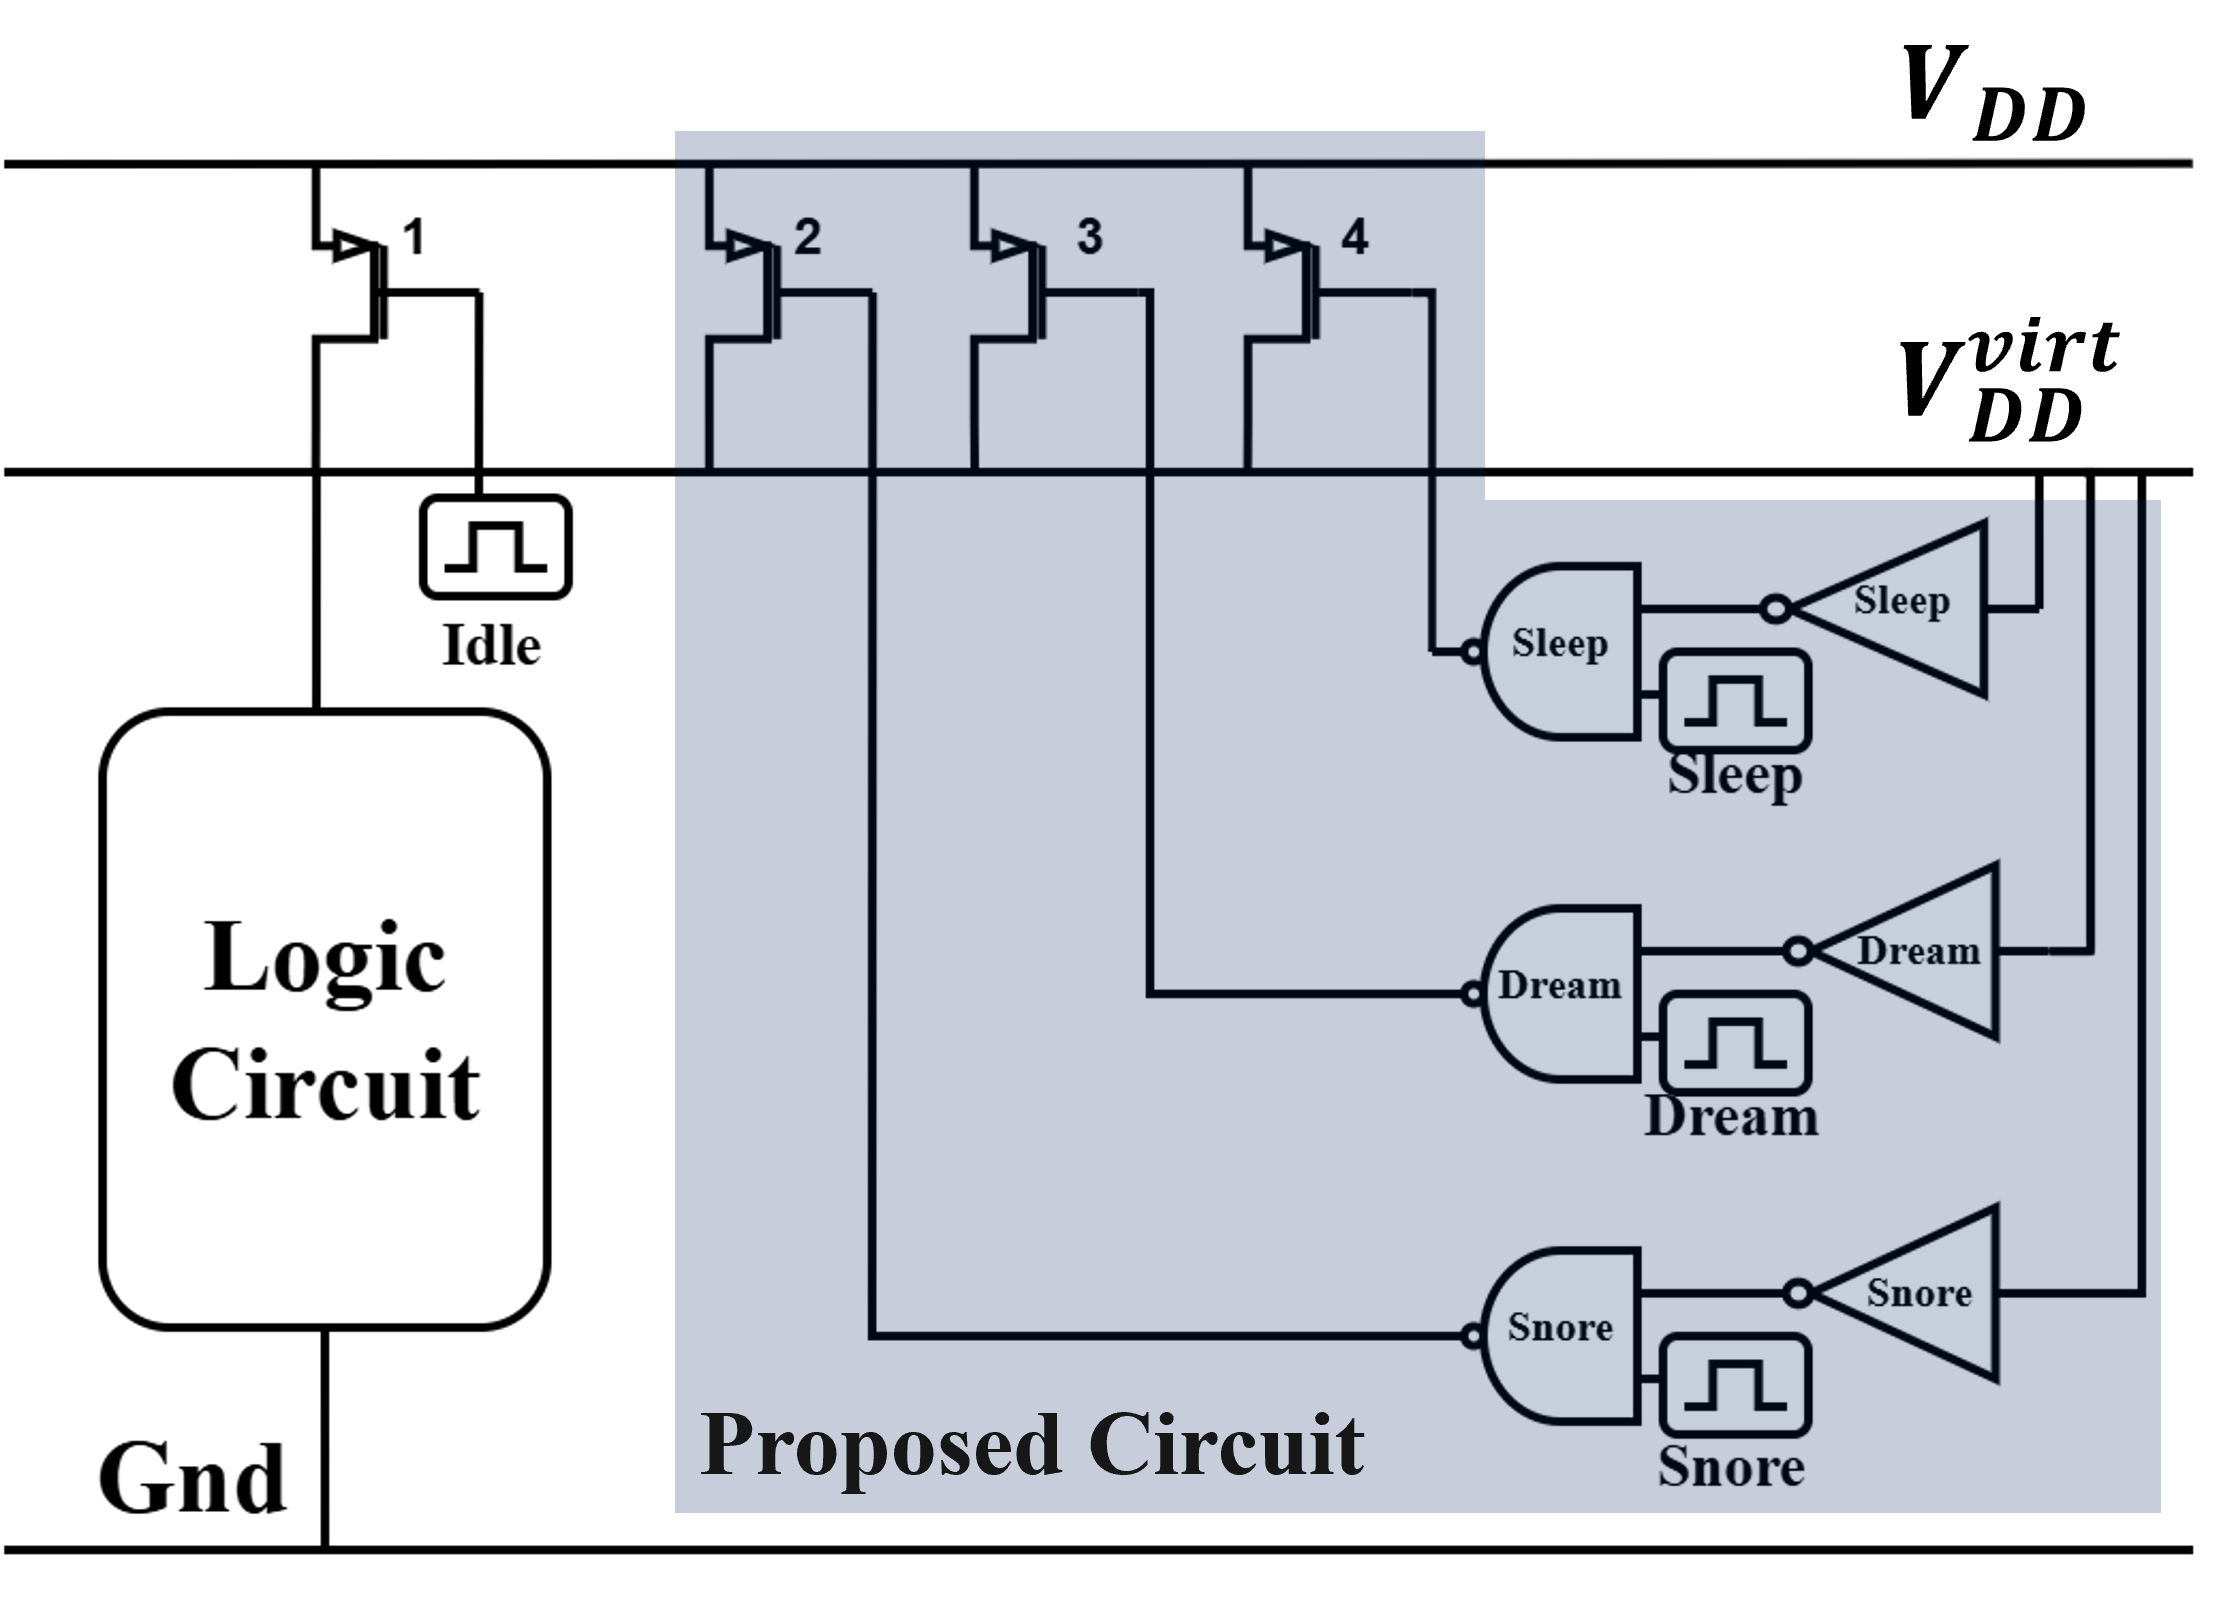
\includegraphics[width=0.45\textwidth]{PG_Ckt_newww.png}
    \caption{Proposed state-retentive multi-sleep mode power gating circuit}
    \vspace{-10pt}
    \label{proposed_PG_Ckt}
\end{figure}

\begin{figure}[t]
    \centering
    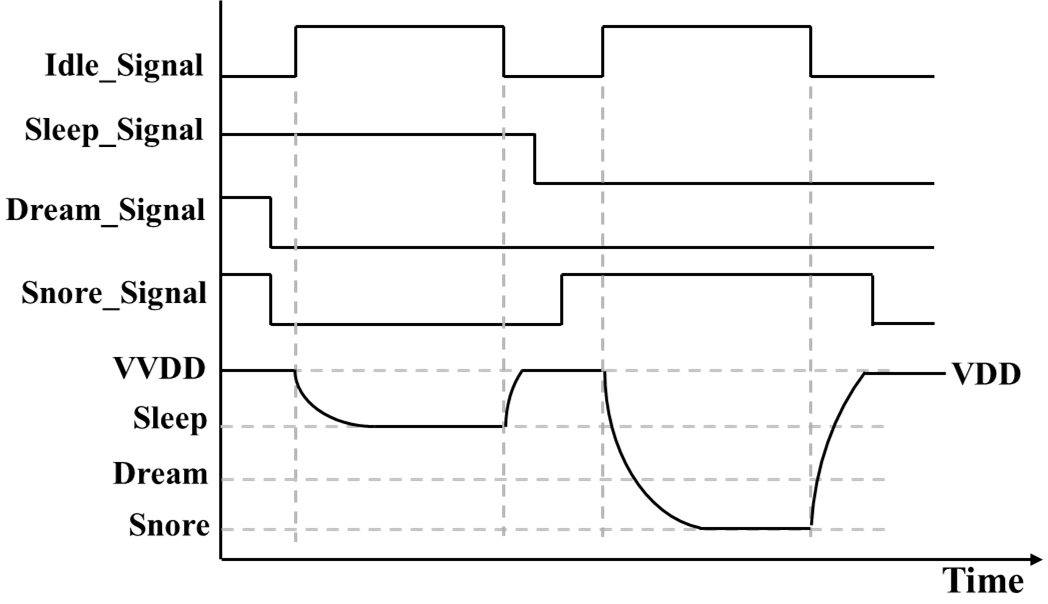
\includegraphics[width=0.4\textwidth]{timing.png}
    \caption{Timing diagram illustrating the dynamic regulation of $V{VDD}$ across sleep, dream, and snore modes}
    \vspace{-10pt}
    \label{timing}
\end{figure}

When the logic circuit's virtual supply voltage ($V_{DD}^{virt}$) is disconnected from the main supply ($V_{DD}$), all internal node voltages—including the gate and drain voltages—are limited to a maximum of $V_{DD}^{virt}$. According to the subthreshold leakage current model~\cite{wang2006subthreshold},

\begin{equation}
    I_{sub} = I_{D0} \times e^{\frac{V_G}{mV_T}} \times (e^{\frac{-V_S}{V_T}} - e^{\frac{-V_D}{V_T}})
\end{equation}
Where, $I_{D0}$ is a technology dependent characteristic current, and $V_G$, $V_S$ and $V_D$ are the gate, source and drain voltages, respectively. $V_T$ is the thermal voltage. Reducing these voltages significantly suppresses the subthreshold leakage current, thereby lowering leakage power.

As illustrated in Fig. \ref{proposed_PG_Ckt}, the proposed circuit regulates the $V_{DD}^{virt}$ across three distinct power gating modes Sleep, Dream, and Snore —each offering a trade-off between leakage power reduction and wake-up latency. Sleep mode provides the shortest wake-up time but the least leakage savings, while Snore mode offers the highest leakage savings at the cost of increased wake-up latency. Dream mode serves as a middle ground, achieving a balanced compromise between the two extremes. Mode selection is managed by a controller implementing a bandit algorithm, which is detailed in the following subsection.

As shown in Fig. \ref{timing}, The controller asserts a logic high ("1") on one of the three mode selection buses, with the other two set to logic low ("0"), thereby indicating the target $V_{DD}^{virt}$ level for the selected mode. Upon detecting an \texttt{Idle\_Signal}, the connection between $V_{DD}$ and $V_{DD}^{virt}$ is disabled through switches 1 and 2, allowing $V_{DD}^{virt}$ to discharge. When $V_{DD}^{virt}$ drops to the voltage level corresponding to a specific mode—identified by the switching threshold of a dedicated inverter—the inverter output transitions to logic high ("1"). This, in conjunction with a logic high from the controller, causes the NAND gate to output logic low ("0"), turning on the corresponding PMOS switch (3 or 4 or 5) and reconnecting $V_{DD}^{virt}$ to $V_{DD}$. As $V_{DD}^{virt}$ charges and surpasses the inverter threshold, the inverter output returns to logic low ("0"), causing the NAND gate to output logic high ("1") and turning off the PMOS switch again. This feedback loop maintains $V_{DD}^{virt}$ at the desired mode-specific level, enabling stable operation within the targeted power gating state.


\subsection{Bandit Algorithm for Adaptive Power Gating Control}
\label{The bandit Algorithm and how it's applied}
The bandit algorithm is a reinforcement learning technique designed to balance exploration and exploitation in sequential decision-making problems. In the context of power gating, selecting an appropriate sleep mode involves a trade-off between leakage energy savings and wake-up latency. Analogous to the multi-armed bandit problem, each power gating mode represents an ``arm'' that yields a certain reward, and the algorithm seeks to maximize the cumulative reward over time.

The reward function is defined as:
\begin{equation}
    \text{Reward} = -(\alpha L_{\text{wakeup}} + \beta E_{\text{leak}})
\end{equation}
where $\alpha$ and $\beta$ are designer-defined weighting coefficients that reflect the relative importance of minimizing wake-up latency $L_{\text{wakeup}}$ and leakage energy $E_{\text{leak}}$. The leakage energy is calculated as $E_{\text{leak}} = P_{\text{leak}} \times t_{\text{idle}}$
with $P_{\text{leak}}$ and $t_{\text{idle}}$ representing the leakage power and idle duration, respectively. The negative sign ensures that minimizing the cost translates into maximizing the reward.

To guide the mode selection process, we employ the Upper Confidence Bound (UCB) algorithm, which selects mode $i$ based on the following criterion:
\begin{equation}
    \text{UCB}_i = \frac{\text{Reward}_i}{n_i} + c \sqrt{\frac{\ln(t)}{n_i}}
\end{equation}
Here, $\text{Reward}_i$ denotes the cumulative reward obtained from mode $i$, $n_i$ represents the number of times mode $i$ has been selected, $t$ is the total number of mode selections across all modes, and $c$ is an exploration coefficient that balances the trade-off between exploration and exploitation. This Upper Confidence Bound (UCB) formulation enables adaptive and intelligent selection of power gating modes. Each time an idle signal is detected, the controller selects the mode with the highest UCB value. Due to the typically homogeneous nature of idle patterns in computing systems—some exhibiting consistently short idle intervals while others experience long idle periods—the algorithm naturally converges to favoring specific modes. For instance, the Sleep mode may be repeatedly selected for short idle durations due to its low wake-up latency, whereas the Snore mode becomes preferable for extended idle intervals owing to its lower leakage power.



\section{Results and Discussion}
This section is organized as follows: In subsection~\ref{3A}, the proposed power gating architecture is evaluated on an SRAM circuit to characterize each mode in terms of leakage power savings and wake-up latency. Subsection~\ref{3B} validates the functionality of the controller integrated with the bandit algorithm, demonstrating its adaptability to various idle patterns. %The controller dynamically selects the appropriate power gating mode based on idle period characteristics and designer-specified preferences for energy savings versus wake-up latency, as determined by the weighting factors in the reward function.

\subsection{Characterization of Power Gating Modes}\label{3A}

\begin{figure}
    \centering
    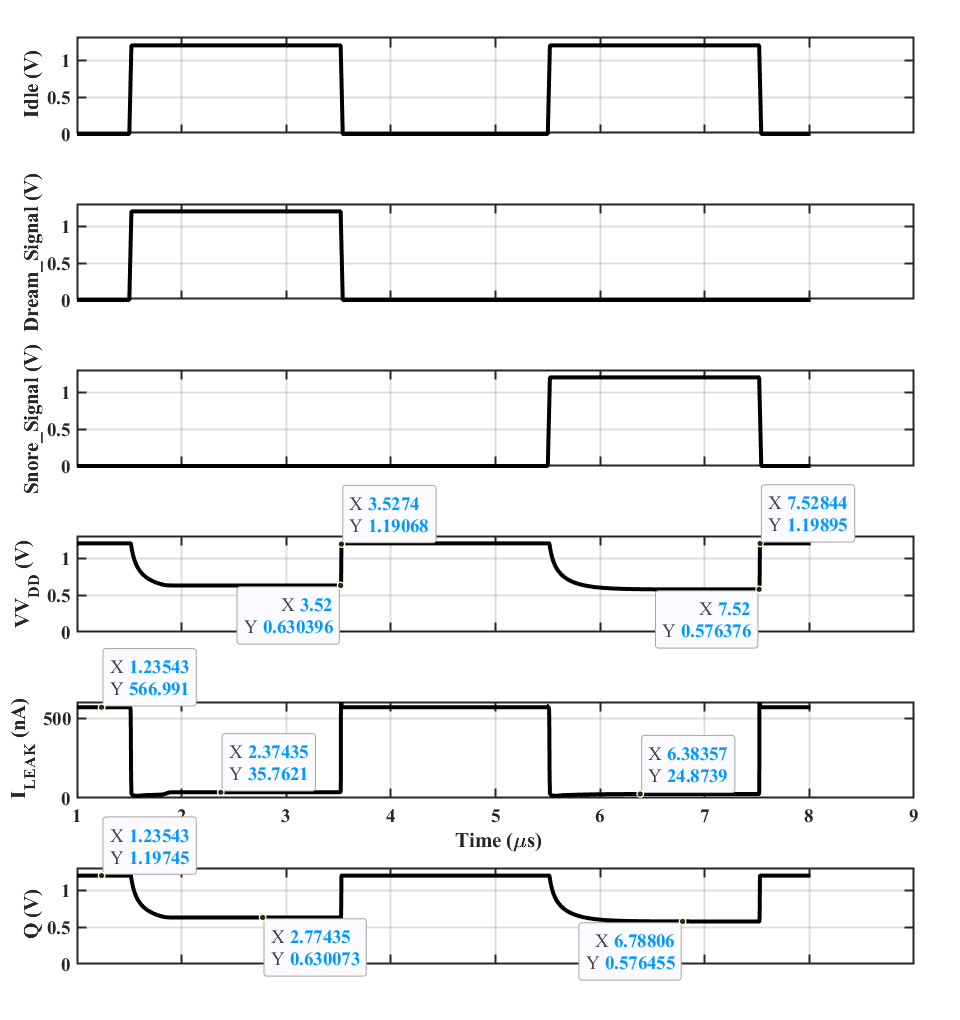
\includegraphics[width=0.9\linewidth]{WAKE_UP_Time_5.png}
    \caption{Transient waveforms showing the idle signal, corresponding leakage current, state retention and virtual supply voltage behavior in different modes.}
    \label{fig:dream_waveforms}
\end{figure}
As shown in Fig.~\ref{fig:dream_waveforms}, when the \texttt{Idle} signal is asserted, the virtual supply voltage ($V_{DD}^{virt}$) begins to drop. With the $Dream\_Signal$ active, $V_{DD}^{virt}$ settles at the Dream inverter threshold (630 mV), reducing the leakage current from 567 nA to 35.76 nA while preserving the SRAM state. The storage node \texttt{Q} scales with $V_{DD}^{virt}$ but is fully restored to $V_{DD}$ upon deassertion of the \texttt{Idle} signal, achieving a wake-up latency of 7.4 ns. In the subsequent idle phase, the  $Snore\_Signal$ is activated, lowering $V_{DD}^{virt}$ further to the Snore inverter threshold (576 mV), resulting in a leakage current of 24.87 nA. Despite the deeper voltage scaling, the SRAM cell retains its state, validating the circuit's effectiveness and robustness.

All modes are evaluated similarly, and key performance metrics—including virtual supply levels, leakage reductions, and wake-up latencies—are summarized in Table \ref{table:sleep_modes}. Leakage power is reduced by 92.5\% to 98\% across sleep to snore modes, respectively. This improvement comes at the cost of increased wake-up latency—from 5.78 ns in sleep mode to 8.1 ns in snore mode. The controller addresses this trade-off by selecting the optimal mode based on idle duration and frequency, using the bandit algorithm to balance energy savings against wake-up latency.

\begin{table}[h]
\centering
\caption{Comparison of Sleep Modes Based on Key Performance Metrics}
\label{table:sleep_modes}
\begin{tabular}{|>{\raggedright\arraybackslash}p{2.5cm}|c|c|c|}
\hline
\textbf{Performance Metric} & \textbf{Sleep mode} & \textbf{Dream mode} & \textbf{Snore mode} \\
\hline
$V_{DD}^{virt}$ (mV)            & 742.5   & 630   & 576 \\
\hline
$I_{leak}$ (nA)              & 69      & 35.76  & 24.87 \\
\hline
$I_{leak}$ reduction (\%)    & 87.83            & 93.7             & 95.6 \\
\hline
$P_{leak}$ (nW)                & 51.23   & 22.53   & 14.32 \\
\hline
$P_{leak}$ reduction (\%)      & 92.5             & 96.68            & 97.9 \\
\hline
Wakeup time (ns)                  & 5.78    & 7.4    & 8.4 \\
\hline
\end{tabular}
\end{table}



\subsection{Validation of the Bandit-Based Power Mode Controller}\label{3B}
\begin{figure}
    \centering
    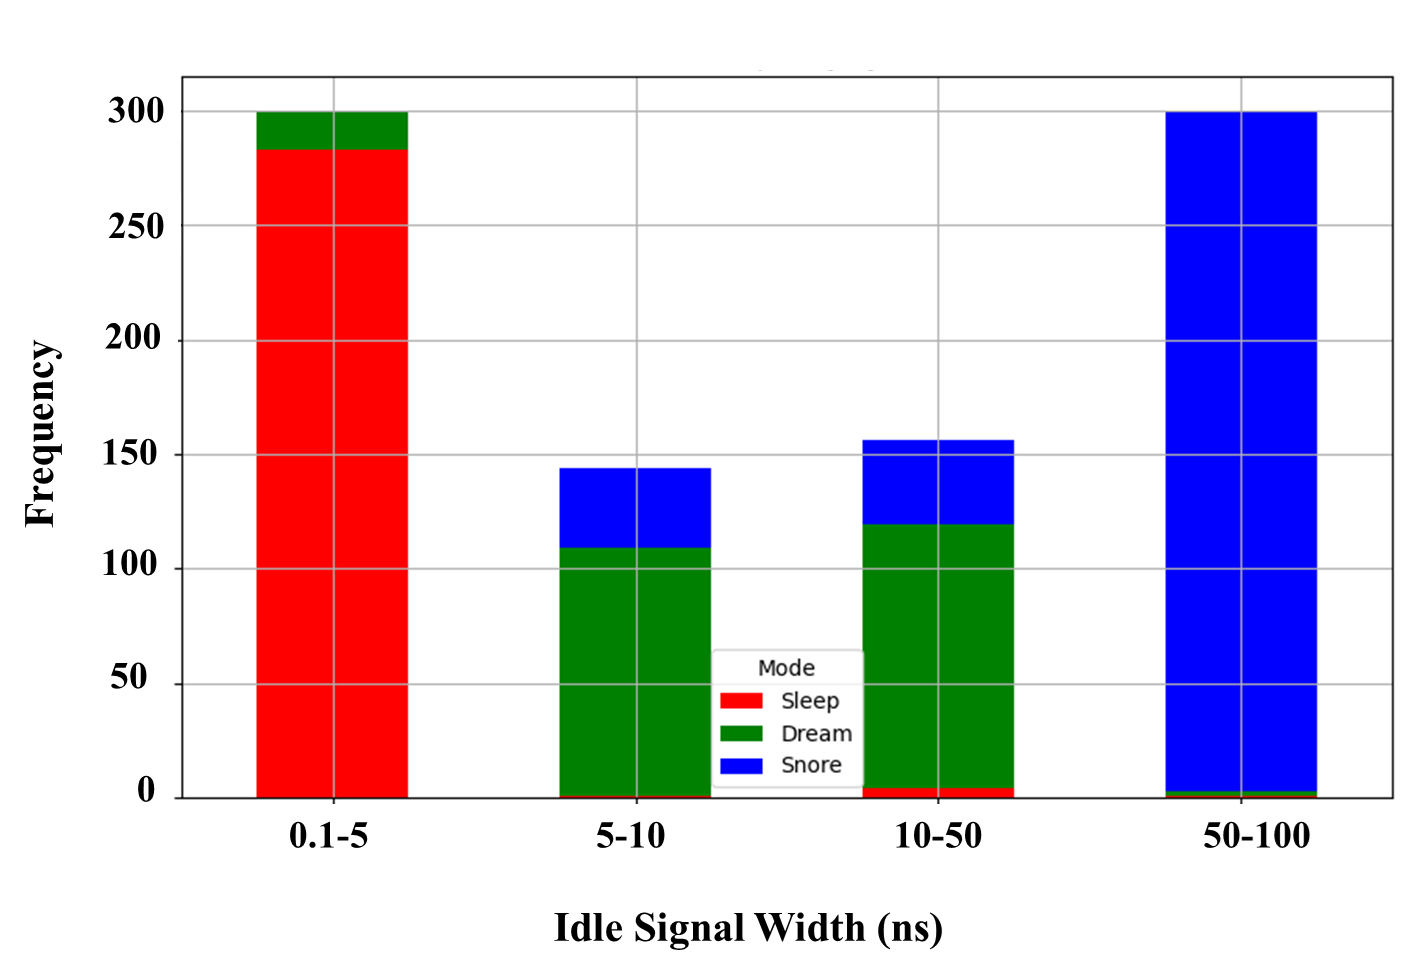
\includegraphics[width=\linewidth]{Bins.png}
    \caption{Mode selection trends relative to idle time intervals}
    \label{Bins}
\end{figure}

To validate the controller, an idle signal pattern of 900 samples was applied, with idle durations ranging from 0.1 ns to 100 ns. When subjected to this periodic and variable idle input, the bandit-based controller initially explores all available power modes and progressively converges toward the mode offering the highest reward—balancing leakage savings and wake-up latency. In this scenario, the controller exhibits a bias toward minimizing wake-up latency. As shown in Fig.~\ref{Bins}, the controller selects the Sleep mode for brief idle intervals, transitions to the Dream mode for medium durations, and opts for the Snore mode during extended idle periods. Some degree of exploration persists within each bin before the controller consistently exploits the optimal mode.

Using this adaptive selection mechanism, the total leakage energy across the test pattern was 0.32 pJ. In contrast, maintaining a single state-retentive mode, as done in \cite{patent} (e.g., Sleep mode only), would have resulted in 1.13 pJ of leakage energy. This demonstrates a 71.7\% further reduction in leakage energy while preserving responsiveness through dynamic mode selection.

\section{Conclusion}
This work presents a low-overhead, multi-mode power gating architecture with a machine learning-based controller that adaptively reduces leakage power in idle-prone systems. Designed in 65 nm CMOS with full state retention, it achieves up to 98\% leakage savings and 71.7\% improvement over SOTA approaches. The solution is robust to process variations and suitable for 2.5D/3D HPC systems.

\vspace{-5pt}


\bibliography{References}
\bibliographystyle{ieeetr}





\end{document}